\documentclass[11pt,english,letterpaper]{scrartcl}


% Used tips from this blog to squish things:
% https://robjhyndman.com/hyndsight/squeezing-space-with-latex/
\usepackage[text={6.5in,9in}]{geometry}
\usepackage{mathptmx}
\setlength{\parskip}{0cm}
\setlength{\parindent}{1em}

%%%%%%%%%%%%%%%%%%%%%%%%%%%%%%%%

% And this is something I found:
\linespread{0.8}

%\usepackage[top=1in, bottom=1in, left=1in, right=1in]{geometry}
\usepackage[T1]{fontenc}
\usepackage[latin9]{inputenc}
\setcounter{secnumdepth}{3}
\setcounter{tocdepth}{2}
\usepackage{color}
\usepackage{babel}

\usepackage[unicode=true, 
pdfusetitle,
bookmarks=true,
bookmarksnumbered=false,
bookmarksopen=false,
breaklinks=true,
pdfborder={0 0 1},
backref=false,
colorlinks=true, urlcolor=blue, linkcolor=blue, citecolor=blue]
{hyperref}

\usepackage{indentfirst}
\usepackage{pgfgantt}

\makeatletter
%%%%%%%%%%%%%%%%%%%%%%%%%%%%%% User specified LaTeX commands.
\usepackage{longtable}
\usepackage{url}
\usepackage{booktabs}
\usepackage{colortbl}
\usepackage{ragged2e}
\usepackage{comment}
\usepackage{pdfpages}
%\usepackage{graphicx}
\usepackage{float}
\usepackage{todonotes}

\makeatother

\begin{document}
\titlehead{DRAFT SERDP FY25 PREPROPOSAL}
\title{Remote Sensing for Detection and Monitoring of Coconut Rhinoceros Beetle Damage}
\author{Prepared by Aubrey Moore PhD, University of Guam (retired)}
%\date{December 17, 2020}

\maketitle

\tableofcontents{}\clearpage{}

\textit{Note to reader: Paragraphs in italics will be removed when the proposal is complete.} \\

\textit{PRE-PROPOSAL LENGTH AND FORMAT: 
Pre-proposals shall be no longer than five (5) pages, type face not less than 11-point, and margins
not less than one inch on all sides.} 

\begin{description}
	
\item[Proposal Number:] \emph{Generated by SEMS when proposal details are entered and saved in the system.}

\item[Proposal Title:] Remote Sensing for Detection and Monitoring of Coconut Rhinoceros Beetle Damage

\item[Lead Principal Investigator:] Roland Quitugua

\item[Lead Organization:] University of Guam, College of Natural and Applied Sciences, Mangilao, Guam

\end{description}

\section{Objective}

\textit{The proposed objectives and how the project is responsive to the objectives
	articulated in the SON.}\\
	
Our objective is to develop an automated remote sensing system that detects, quantifies and monitors coconut rhinoceros beetle (CRB) damage on isolated Pacific islands using artificial intelligence (AI) to scan georeferenced digital images. This system will use images acquired from several sources, including roadside surveys, aerial drone surveys and the worldwide web.

This proposal addresses the statement of need (SON) entitled \textit{Advancing Non-Indigenous Invasive Species Surveillance, Mitigation, or Biosecurity Measures Affecting Military Readiness in the Indo-Pacific Region}. The objective of this SON "is to solicit proposals that develop and mature the science to detect, survey, mitigate, characterize impacts, and minimize the establishment or spread of invasive species in the Indo-Pacific region".

\todo[inline]{Show how the project is responsive to the objectives
	articulated in the SON}

\section{Background}

\textit{Sufficient technical background to demonstrate a thorough understanding of the problem and frame the proposed research in the context of the current state of the science or technology.}\\

Coconut rhinoceros beetle (CRB), \textit{Oryctes rhinoceros}, is one of the most problematic invasive species in the Indo-Pacific region. This beetle is endemic to the tropical Asia region (including South East Asia). CRB damages both coconut and oil palm, and can sometimes kill palms when adults bore into crowns to feed on sap \cite{Bedford2013} (Bedford, 2013a, 2013b). The beetle was inadvertently introduced into the Pacific in 1909 when infested rubber tree plants were transported to Samoa from Sri Lanka (previously known as Ceylon) (Catley, 1969). The pest rapidly multiplied in Samoa and subsequently spread to several nearby Polynesian islands. Separate invasions further distributed CRB through Palau, parts of Papua New Guinea, and other Pacific nations through disruptions and uncontrolled movements during World War II (Catley, 1969; Gressitt, 1953). The invasive phase of the beetle was brought under control by the discovery and distribution of a viral biocontrol agent, \textit{Oryctes rhinoceros} nudivirus (OrNV). OrNV is currently present and causes persistent population suppression on many of the CRB infested Pacific Islands (Bedford, 2013b; Huger, 2005). Virus introduction into affected Pacific Island countries and territories suppressed and weakened the CRB populations such that its spread into the Pacific islands ceased and for 30 years there was no further range expansion of CRB (Secretariat of the Pacific Community, 2015). 

\todo[inline]{replace following with table}

However, the situation changed following discovery of an OrNV resistant CRB population on Guam in 2007 \cite{Marshall2017}. Since 2007, CRB has invaded the Hawaiian Islands ( (Oahu in 2013, Kauai in 2023, Big Island in 2023), Commonwealth of the Northern Mariana Islands (Rota ????), Republic of the Marshall Papua New Guinea (Port Morseby area in ????), Solomon Islands (Guadalcanal in ????, Savo in ????, Malaita in ????; and Rota (Commonwealth of the Northern Mariana Islands). Beetles in the third wave of invasions are genetically different from those in the earlier waves and these are being referred to as the Guam biotype or CRB-G.



However, the situation changed following discovery of an OrNV resistant CRB population on Guam in 2007 \cite{Marshall2017}, this pest has resumed its spread throughout the Pacific. Recently invaded islands include Guam (2007) ... Majuro, RMI (2023), Kauai, HI (2023), Hawaii, HI (2023).

\subsection{CRB damage survey methods}

V-shaped cuts to palm fronds and other symptoms of CRB adult feeding activity are highly distinctive and visible from up to a few hundred meters.

A review of CRB damage survey methods is provided by \cite{Mansfield2023}. Recent surveys almost always use georeferenced digital images. Severity of damage to palms in these images is later classified by human experts using a standardized 3-level scale (undamaged, damaged, dead) or a 5-level scale (undamaged, low damage, medium damage, high damage, dead). Results are then displayed on a map. 

\subsection{Automation of CRB damage surveys}

On Guam, CRB damage surveys have been automated in three ways:
Images are not taken by a human, but are taken by a smart phone camera which snaps photos at a rate of one per second and records GPS coordinates;
Coconut palms in each image are located, assigned a damage level, and are scanned for v-shaped cuts by AI object detectors;
Location of coconut palms and damage levels are automatically added to an interactive web map.
This allows us to complete a damage survey of Guam within the few hours it takes to drive all the major roads on the island in both directions.

\subsection{Images of CRB damage on the world-wide-web}

Images of coconut palms with probable CRB damage are publicly available on the world-wide-web. Some of these are the result of citizen science projects initiated specifically to detect CRB damage, such as \href{https://www.inaturalist.org/projects/retired-fa-15-uog-crb-damage-survey}{an iNaturalist project entitled \textit{FA 15 UOG CRB Damage Survey}} and a \href{https://www.projectnoah.org/missions/182566002}{Project Noah mission entitled \textit{Help Save Hawaii's Coconut Trees}}.

In addition, there are many unlabeled images of coconut palms available as incidental images within social media and elsewhere on the world-wide-web and new images are being added daily. Paudel and Jackson have been tracking potential biosecurity incursions using publicly available images on the web \cite{Paudel2023} and have discovered strong evidence that CRB has invaded Mexico \cite{Jackson2022}.

We intend to apply our object detectors to automate searches for CRB damage in publicly available images on the web.

\subsection{Previous work on automated CRB damage surveys}
\label{previous_work}
The proposed project builds on an existing system which maps CRB damage using automated analysis of ground-based imagery which uses a smart phone mounted on a road vehicle for data acquisition. Currently, images are taken at a rate of one per second by a free cell phone app named OpenCamera. Each image is 1920 x 1080 pixels in size and GPS coordinates are embedded within the image file. Note that the phone does not require a SIM card or internet connection during data acquisition. 

After transferring image files to a laptop computer, each is examined by a pair of object detectors trained by an artificial intelligence technique called deep learning. One detector puts a bounding box around all coconut palms within each image and assigns a standardized 5-scale damage index to each palm [REF]. The damage index is based on a standard methodology developed by CRB experts working on islands in the south Pacific [REF]. A second object detector counts v-shaped cuts to coconut palm in fronds which are distinctive signs of CRB feeding damage. Results are visualized using interactive web maps. This ground-based system has been used for routine roadside surveys on Guam and has also been used for early detection of CRB damage on Rota in the Commonwealth of the Northern Mariana Islands and on Majuro in the Republic of the Marshall Islands [REFS].

For details on this ground-based CRB damage survey methodology see the attached file roadside.pdf.

We will improve the existing ground-based system and adapt this system to use aerial drone imagery to facilitate:
\begin{itemize}
	\item CRB damage detection over large areas of remote, otherwise inaccessible, terrain
	\item early detection and delimiting surveys in rapid response projects on islands where CRB has not yet established, increasing chances of eradication
	\item monitoring temporal and spatial changes in CRB damage on islands where CRB has	established
	\item measuring changes in CRB damage in response to biological control, sanitation, and other mitigation tactics
\end{itemize}

\section{Approach}

\textit{The technical approach and methods, preferably structured in hypothesis-driven tasks that clearly identify how the objectives of the proposed project will be addressed. This section should be the primary focus of the pre-proposal.}

\paragraph{Design considerations.} All code will be developed using free open-source software (FOSS) and all code, data and documentation generated by the project will be made available via public GitHub repositories.

\paragraph{Object detectors.} Existing object detectors, which have been used in roadside CRB damage surveys on Guam since 2020, will be retrained to minimize false positives and false negatives. Performance before and after retraining will be evaluated using standard metrics and reported in a technical report. A user manual will also be provided. 

\paragraph{Roadside surveys.} Improved object detectors will be tested in quarterly CRB damage surveys on Guam using \hyperref[previous_work]{methods detailed above}. Combined roadside and drone surveys are planned for Majuro. 

\paragraph{Aerial drone surveys.} Object detectors will be retrained to detect CRB from the air. High quality aerial dataset of drone imagery acquired specifically for this purpose on Guam is available [REF]. An initial field trial of the drone survey methodology will be conducted on Guam. Technical documentation and a user guide for the aerial drone survey methodology will be written. Operational testing be performed on Majuro.

\paragraph{World wide web surveys.}

Our object detectors can process images acquired from the world-wide-web.


\begin{itemize}
	
	\item improve ground-based system
	\begin{itemize}
		\item improve code to minimize false positive s and false negatives
		\item evaluate performance using standard metrics
		\item provide technical documentation
		\item provide user manual
		\item develop and test a cell phone app which does real-time object detection. This can be done by embedding the two object detectors in the app. This app would work in much the same way as a license plate reader: sending out an alert whenever CRB damage is detected. Images to be saved for eventual upload and further analysis. IF THIS APP IS MADE AVAILABLE PUBLICLY, IT COULD BE USED FOR CROWD SOURCED DATA SIMILAR TO INAT.
	\end{itemize}
	
	\item develop aerial-based system
	\begin{itemize}
		\item train object detectors to detect CRB damage from aerial images using the existing VDC orthomosaic
		\item evaluate performance using standard metrics
		\item provide technical documentation
		\item provide user manual
	\end{itemize}
	
	\item operational testing
	\begin{itemize}
		\item initial operational testing of the ground-based system during routine island-wide CRB damage surveys on Guam
		\item initial operational testing of the aerial-based system using new imagery from VDC
		\item remote operational testing on Majuro: ground-based system for roadside survey; aerial-based survey for islets in the northern part of the atoll
		\item detection survey on Kiribati using both ground-based and aerial-based methods		
	\end{itemize}
	
\end{itemize}

\section{Schedule}

\textit{The duration of the project, along with a milestone chart that delineates the timeline for each task and major deliverables.} \\

The duration of this project component will be 4 years. A schedule with milestones is provided as Fig. \ref{fig:gantt}.

\begin{figure}[h!]
	%\centering
	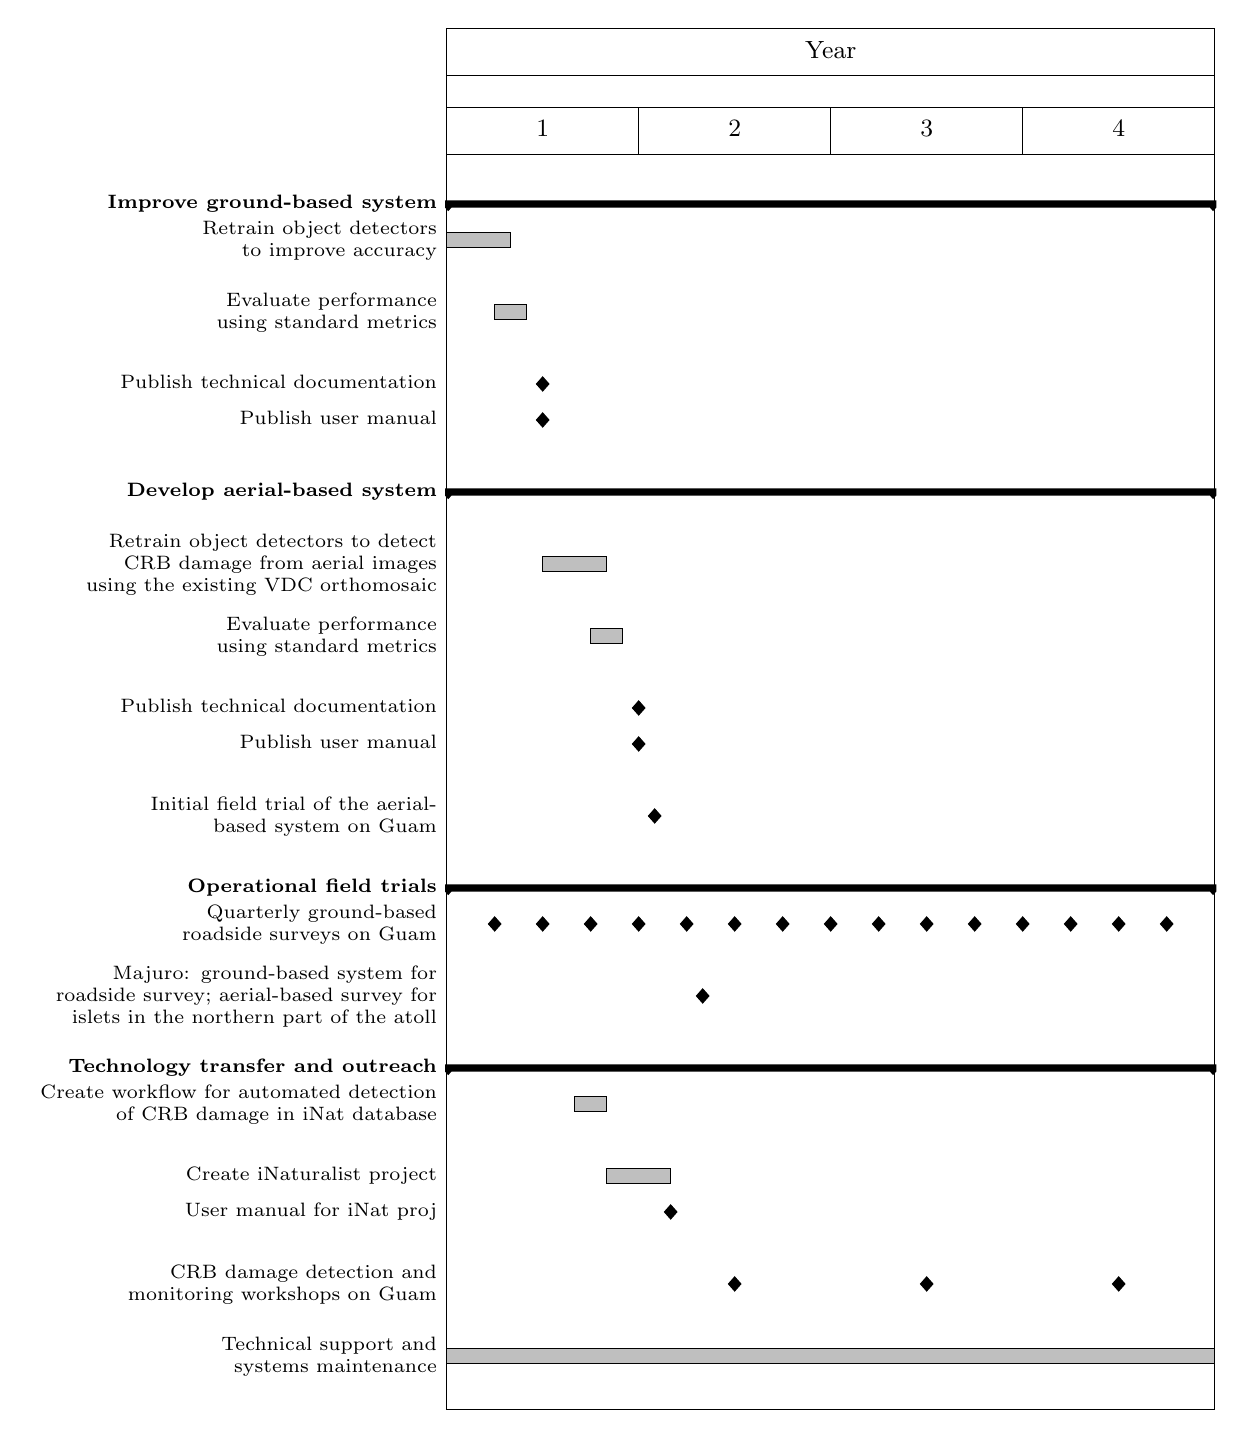
\begin{tikzpicture}
	\begin{ganttchart}[x unit=0.08in, 
	y unit chart=0.18in,
	group label node/.style={text width=2in,align=right,font=\scriptsize\RaggedLeft,anchor=east},
	bar label node/.style={text width=2in,align=right,font=\scriptsize\RaggedLeft,anchor=east},
	milestone label node/.style={text width=2in,align=right,font=\scriptsize\RaggedLeft,anchor=east},
	bar/.append style={fill=lightgray}
	]{1}{48}
	
	\gantttitle{Year}{48} \\
	\gantttitlelist{1,...,4}{12} \\
	
	\ganttgroup{\textbf{Improve ground-based system}}{1}{48} \\
		\ganttbar{Retrain object detectors to improve accuracy}{1}{4} \\\\
		\ganttbar{Evaluate performance using standard metrics}{4}{5} \\\\		
		\ganttmilestone{Publish technical documentation}{6} \\
		\ganttmilestone{Publish user manual}{6} \\\\
		
	\ganttgroup{\textbf{Develop aerial-based system}}{1}{48} \\\\
		\ganttbar{Retrain object detectors to detect CRB damage from aerial images 		using the existing VDC orthomosaic}{7}{10} \\\\
		\ganttbar{Evaluate performance using standard metrics}{10}{11} \\\\
		\ganttmilestone{Publish technical documentation}{12} \\
		\ganttmilestone{Publish user manual}{12} \\\\
		\ganttmilestone{Initial field trial of the aerial-based system on Guam}{13} \\\\
		
	\ganttgroup{\textbf{Operational field trials}}{1}{48} \\
		\ganttmilestone{Quarterly ground-based roadside surveys on Guam}{3}			
			\ganttmilestone{}{6}
			\ganttmilestone{}{9}
			\ganttmilestone{}{12}
			\ganttmilestone{}{15}
			\ganttmilestone{}{18}
			\ganttmilestone{}{21}
			\ganttmilestone{}{24}
			\ganttmilestone{}{27}
			\ganttmilestone{}{30}
			\ganttmilestone{}{33}
			\ganttmilestone{}{36}
			\ganttmilestone{}{39}
			\ganttmilestone{}{42}
			\ganttmilestone{}{45} \\\\		
		\ganttmilestone{Majuro: ground-based system for roadside survey; aerial-based survey for islets in the northern part of the atoll}{16} \\\\
	
	\ganttgroup{\textbf{Technology transfer and outreach}}{1}{48} \\
		\ganttbar{Create workflow for automated detection of CRB damage in iNat database}{9}{10} \\\\
        \ganttbar{Create iNaturalist project}{11}{14} \\
        \ganttmilestone{User manual for iNat proj}{14} \\\\
        \ganttmilestone{CRB damage detection and monitoring workshops on Guam}{18}
        \ganttmilestone{}{30}
        \ganttmilestone{}{42} \\\\
        \ganttbar{Technical support and systems maintenance}{1}{48} \\        
	
	\end{ganttchart}	
	\end{tikzpicture}
	\caption{Project schedule.} 
	\label{fig:gantt}
\end{figure}




%\textit{The duration of the project, along with a milestone chart that delineates the timeline for each task and major deliverables.}


%\begin{figure}[h]
%	\includegraphics[width=\textwidth]{ProjectLibre/gantt.png}
%	\caption{Project schedule. This screenshot is a placeholder. Will be replaced with the real thing.}
%\end{figure} 


\begin{comment}

Major benchmarks are:

\begin{enumerate}
	\item \textbf{Discovery of an OrNV isolate which can be used as an effective biological control agent for CRB-G.} Candidate isolates will be evaluated in laboratory bioassays.
	\item \textbf{Release of OrNV into populations by autodissemination.} Laboratory facilities will be established to produce selected OrNV isolates \textit{in vivo} and/or \textit{in vitro}. 
	\item \textbf{Establishment of self sustaining biological control which prevents significant damage from CRB-G on an island-wide basis} Progress towards this goal will be assessed by a periodic damage monitoring survey will be established prior to release of biocontrol agents. 
\end{enumerate}

	
From PPA20:

Milestones:

Objective 1:  Establish Sustainable CRB-G Biocontrol by Autodissemination of OrNV

Month 1,2,3,4,5,6: Introduce OrNV biological control candidates into the Guam CRB-G population by autodissemination.

Month 2: Establish a breeding colony for CRB-G and CRB-S.

Month 3,4,5,6: Perform laboratory bioassays to measure differences in responses to OrNV by CRB-G and CRB-S. In addition to mortality, we will measure differences in oviposition and flight capacity.

Month 7, 8: Perform y-tube olfactometer trials to test for differences in attraction to oryctalure by CRB-G and CRB-S.

Month 7,8,9,10,11: Perform surveys to measure spread of OrNV within the Guam CRB-G population.

Month 12: Prepare final report.

Objective 2:  Establish a Sustainable Coconut Palm Health Monitoring System

Months 1,3,5,7,9,11: Island-wide roadside surveys will be done bimonthly using images recorded using an Olympus TG5 camera equipped with a GPS receiver mounted on a vehicle.

Month 1: Annotate videos using the Computer Vision Annotation Tool (CVAT).

Month 2: Use annotations to train an object detector for CRB damage using the Faster R-CNN model implemented in the TensorFlow object detection API. This work requires setting up a virtual machine with graphics processing unit (GPU).

Month 3: Evaluate results from the trained object detector. If precision is insufficient, collect more annotated videos and add these to the training set.

Month 4: Develop a software system which will take raw video GPS tracks as input, outputting CRB damage maps and statistics.

Month 12: Prepare final report.

\end{comment}

\section{Cost}

\textit{The estimated total costs, including labor, materials, travel, burdens, and profit	(fixed fee, if any, for eligible organizations) by year. A detailed breakout of costs is not	required or desired in the pre-proposal.}\\

Estimated total costs for this project component are provided in Table \ref{sec:cost-breakdown}.

\begin{table}[h]
	\centering
	\caption{Summary of project cost estimates.
		Indirect rates are 26\% for CEMML, 27.6\% for NCSU, and 15\% for UOG.
		These rates are applied to Labor + Materials + Travel.
		In addition, NCSU charges 27.6\% on the first \$25k of each subcontract awarded to CEMML and UOG. For details see Appendix~\ref{sec:cost-breakdown}.}	
%	
\begin{tabular}{llrrrrrr}
\toprule
Year & Institution & Labor & Materials & Travel & Rent & Indirects & Year total \\
\midrule
1 & CEMML & \$145,618 & \$29,102 & \$11,817 & \$12,000 & \$48,499 & \$247,036 \\ 
1 & NCSU & \$33,959 & \$0 & \$37,000 & \$1,000 & \$33,384 & \$105,343 \\ 
1 & UOG & \$378,980 & \$96,250 & \$0 & \$0 & \$71,284 & \$546,514 \\ 

    \midrule    
    1 & All & \$558,557 & \$125,352 & \$48,817 & \$13,000 & \$153,167 & \$898,893 \\ 

    \midrule
    2 & CEMML & \$149,985 & \$28,102 & \$0 & \$12,000 & \$46,302 & \$236,389 \\ 
2 & NCSU & \$44,677 & \$0 & \$50,000 & \$1,000 & \$39,930 & \$135,607 \\ 
2 & UOG & \$397,041 & \$56,250 & \$0 & \$0 & \$67,993 & \$521,284 \\ 

    \midrule    
    2 & All & \$591,703 & \$84,352 & \$50,000 & \$13,000 & \$154,225 & \$893,280 \\ 

    \midrule
    3 & CEMML & \$154,484 & \$26,102 & \$0 & \$12,000 & \$46,952 & \$239,538 \\ 
3 & NCSU & \$36,432 & \$0 & \$50,000 & \$1,000 & \$37,655 & \$125,087 \\ 
3 & UOG & \$408,952 & \$56,250 & \$0 & \$0 & \$69,780 & \$534,982 \\ 

    \midrule    
    3 & All & \$599,868 & \$82,352 & \$50,000 & \$13,000 & \$154,387 & \$899,607 \\ 

    \midrule
    4 & CEMML & \$158,921 & \$26,102 & \$0 & \$12,000 & \$48,105 & \$245,128 \\ 
4 & NCSU & \$43,853 & \$0 & \$36,000 & \$1,000 & \$35,839 & \$116,692 \\ 
4 & UOG & \$408,033 & \$56,250 & \$0 & \$0 & \$69,642 & \$533,925 \\ 

    \midrule    
    4 & All & \$610,807 & \$82,352 & \$36,000 & \$13,000 & \$153,586 & \$895,745 \\ 

    \midrule
    
\bottomrule
\end{tabular}

	\label{tbl:cost}
\end{table}

\section{Research Team}

\textit{Identify the Principal Investigator(s), the key co-performers, and their respective organizations. If multiple co-performers are proposed, indicate their responsibilities within the project.}\\

The members of the research team for this project component and their roles are listed in Table \ref{tbl:team}.

\begin{table}[h]
	\centering
	\caption{Research team and roles.}	
	
	\begin{tabular}{p{2.2in}p{4in}}
		\toprule
		\textbf{Research team members} & \textbf{Roles} \\ \midrule
		
		Roland Quitugua (PI), University of Guam & Project management \\ \midrule
		
		Dr. Aubrey Moore, University of Guam (retired) & Systems design and coding \\ \midrule
		
		Dr. Romina King, University of Guam & Drone imagery and GIS \\ \midrule
		
		Dr. Ken Puliafico, Center for Environmental Management of Military Lands, Colorado State University & Liaison with DOD and CRB damage surveys on DOD lands in Guam. \\ \midrule
		
		Dr. Mark Ero, Secretariat of the Pacific Community, Fiji & \\ \midrule
		
		Dr. Sulav Paudel, AgResearch New Zealand & \\ \midrule
		
		Dr. Sean Marshall, AgResearch, New Zeland, Fiji & \\ \bottomrule	
		
	\end{tabular}
	\label{tbl:team}
	
\end{table}

\begin{table}[h]
	\centering
	\caption{List of additional collaborators, not directly funded by this project. TO BE POPULATED.}	
	
	\begin{tabular}{p{2.2in}p{4in}}
		\toprule
		\textbf{Collaborator(s)} & \textbf{Roles} \\ \midrule
		
		Name(s) and affiliation & Roles \\ \midrule
				
	\end{tabular}
	\label{tbl:team-additional}	
\end{table}



\clearpage

\appendix

\newpage

\section{Abbreviated Curriculum Vitae}

\textit{Required: One (1) page each for the Principal Investigator and other significant performers involved with the project that provide relevant research experience. Include the full mailing addresses, phone numbers, and email addresses for each person listed.}

\subsection{Roland Quitugua}
COMING SOON.

\subsection{Dr. Aubrey Moore}
Please see next page.
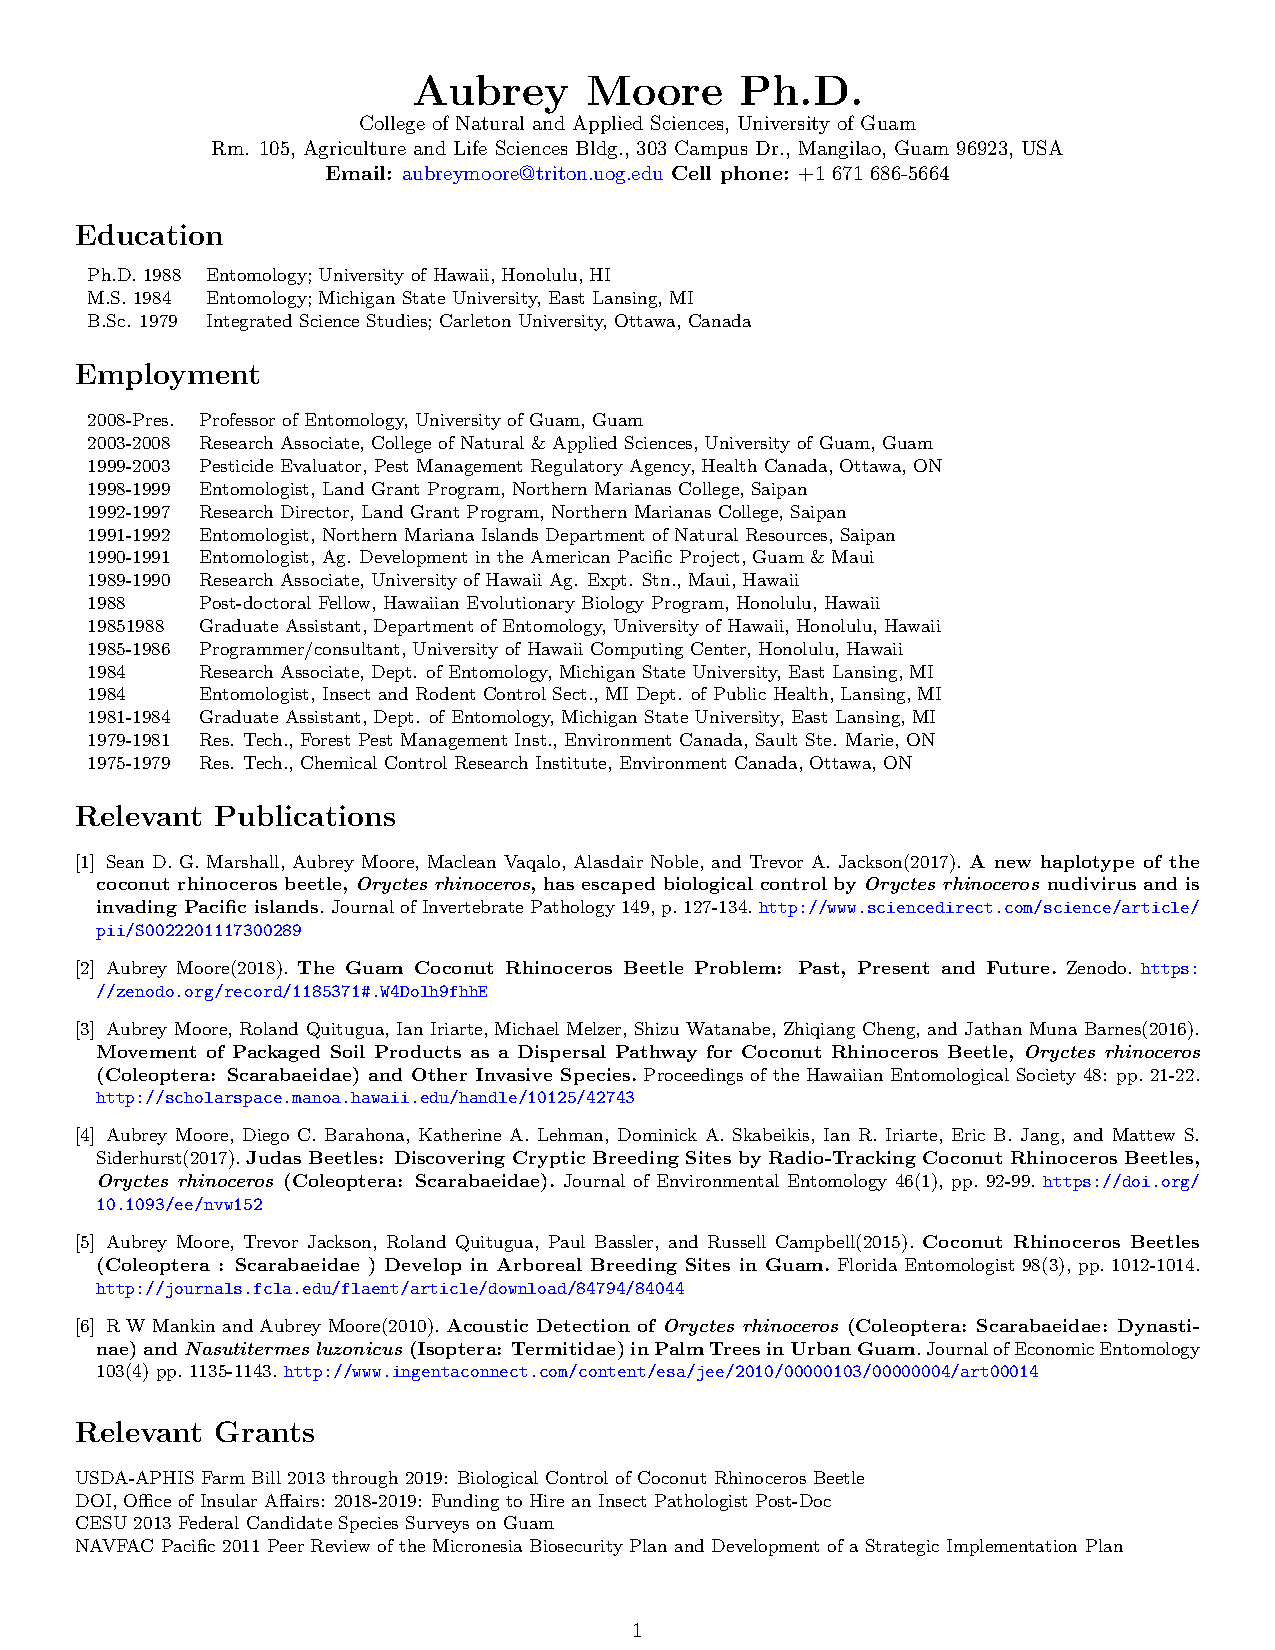
\includepdf[pages=-]{vitae/aubrey-moore-cv.pdf}

\subsection{Dr. Romina King}
COMING SOON.

\subsection{Dr. Kenneth Puliafico}
Please see next page.
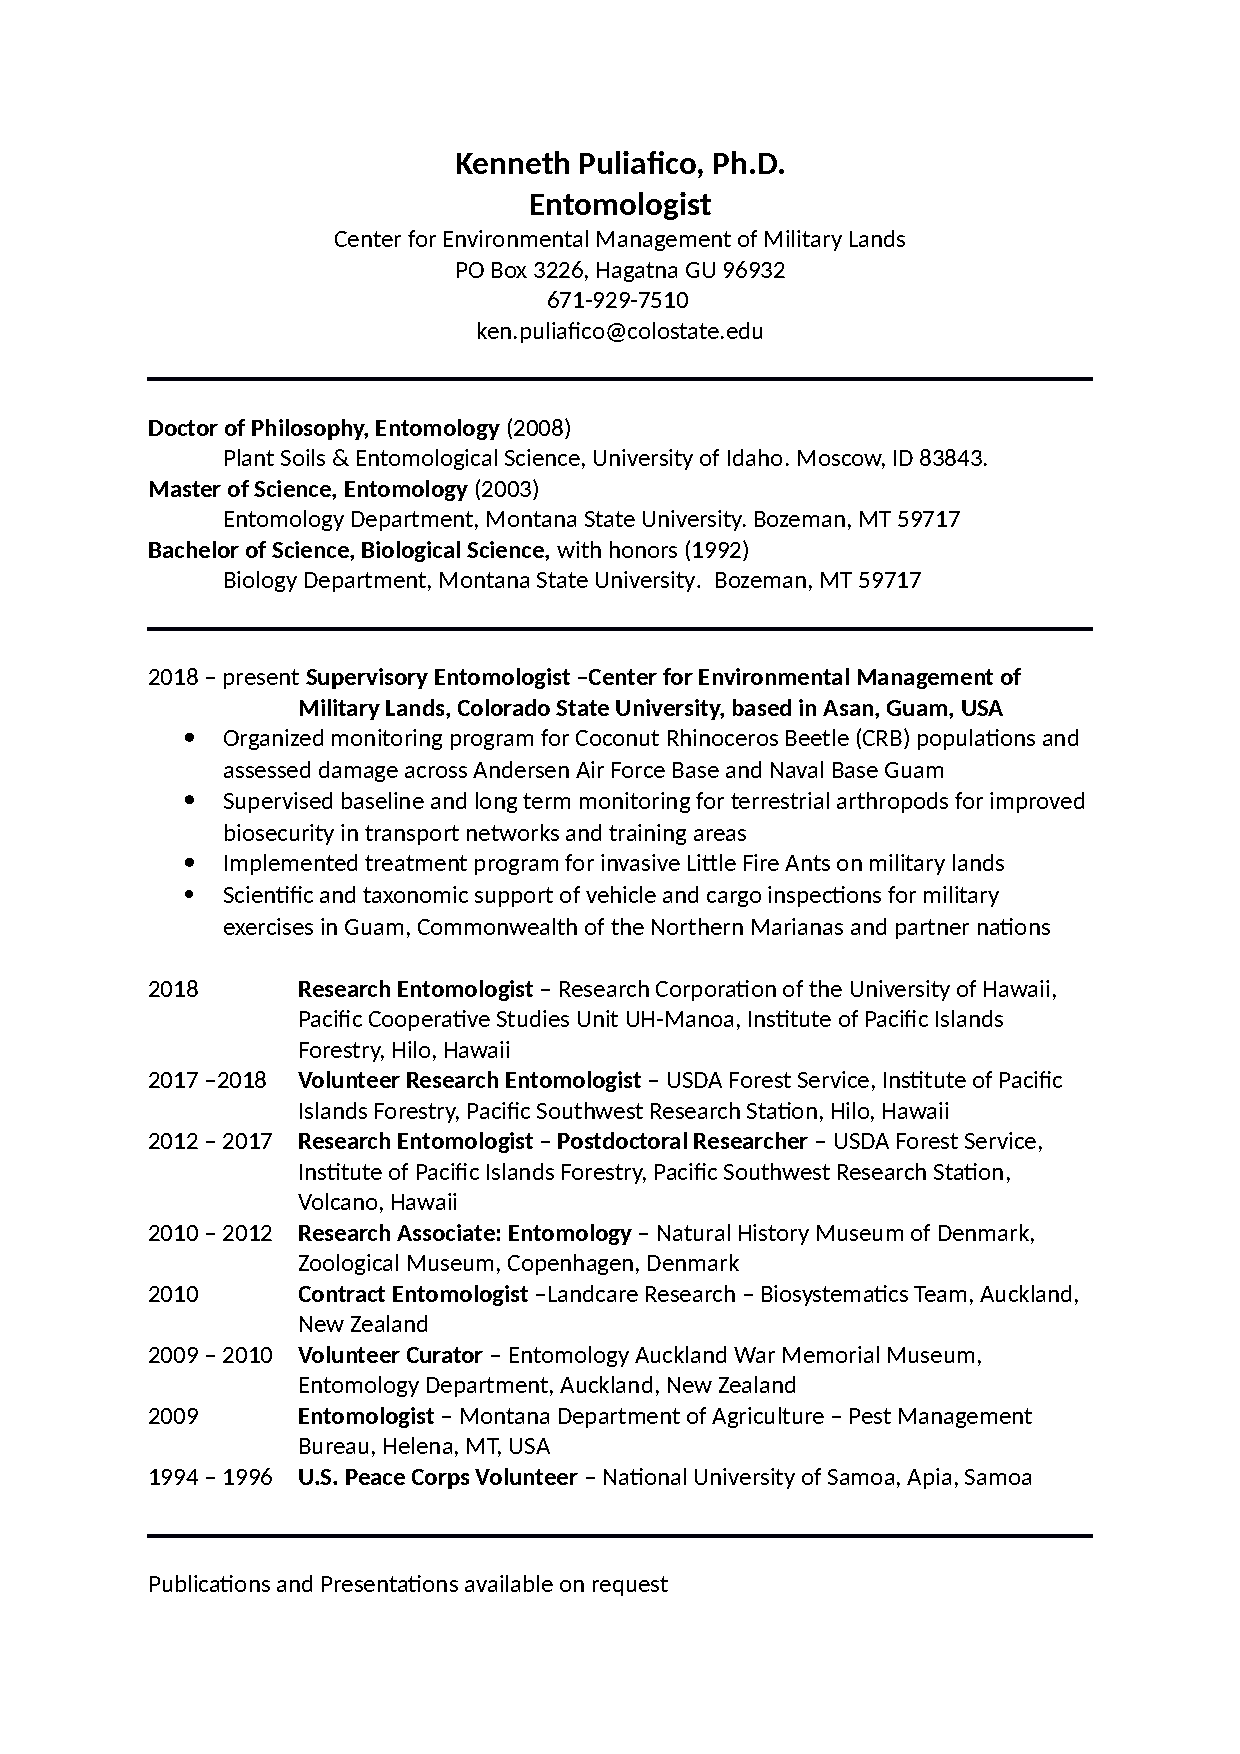
\includepdf[pages=-]{vitae/Puliafico.pdf}

\subsection{Dr. Mark Ero}
COMING SOON.

\subsection{Dr. Sulav Paudel}
COMING SOON.

\subsection{Dr. Sean Marshall}
COMING SOON.

\section{List of Acronyms}

\textit{Required: Provide a complete list of acronyms used in your preproposal and their definitions. List the proposal number at the top of the page.} \\

\begin{description}
	\item[Proposal Number:] \emph{Proposal Number: Generated by the SERDP and ESTCP Management System (SEMS) when the proposal details are entered and saved in the system.}
\end{description}

\begin{description}
	\item[CEMML] Center for Environmental Management of Military Lands, Colorado State University
	\item[CRB] Coconut rhinoceros beetle, \textit{Oryctes rhinoceros}
	\item[CRB-G] Coconut rhinoceros beetle, Guam biotype
	\item[CRB-S] Coconut rhinoceros beetle, not Guam biotype
	\item[DOD] United States Department of Defense
	\item[IATS] Invasive, alien terrestrial species
	\item[LD50] Dose which causes 50\% mortality
	\item[LT50] For a fixed dose, this is time between treatment and 50\% mortality
	\item[NCSU] North Carolina State University
	\item[OrNV] \textit{Oryctes rhinoceros} nudivirus, a biological control agent for coconut rhinoceros beetle
	\item[SON] Statement of need
	\item[USDA-APHIS] United States Department of Agriculture, Animal \& Plant Health Inspection Service
\end{description}

\clearpage

\section{Literature Citations}

\textit{Required, if literature is cited: Literature Citations: Provide literature citations for any material cited in the technical section or the supporting technical data.} \\

\begingroup
\renewcommand{\section}[2]{}% Gets rid of the References header
\begin{thebibliography}{1}
	
\bibitem{Jackson2022} Jackson TA, Rincon M, Villamizar L, Paudel S (2022). Social media posts suggest that coconut rhinoceros beetle has established in the Western Hemisphere. \url{https://doi.org/10.22541/au.165828152.28371110/v1}
	
\bibitem{Paudel2023} Paudel S, Jackson TA (2023). Tracking potential biosecurity incursions using publicly available images: A case of coconut rhinoceros beetle. Journal of Applied Entomology, 147(8), 661?666. 
\url{https://doi.org/10.1111/jen.13155}
	
\bibitem{Mansfield2023} Mansfield S, Balanama A, van Koten C, Paudel S, Bowie M, Jackson TA, Marshall SDG (2023). Assessment of coconut palm damage caused by coconut rhinoceros beetle, \textit{Oryctes rhinoceros} (Coleoptera: Scarabaeidae), New Zealand Journal of Crop and Horticultural Science \url{https://doi.org/10.1080/01140671.2023.2278791}
	
%\bibitem{Bedford1986} Bedford G. O. (1986). Biological control of the rhinoceros beetle (\textit{Oryctes rhinoceros}) in the South Pacific by baculovirus. Agriculture, Ecosystems and Environment. 15:141-7.

\bibitem{Bedford2013} Bedford, G. O.(2013). Long-term reduction in damage by rhinoceros beetle \textit{Oryctes rhinoceros} (L.) (Coleoptera: Scarabaeidae: Dynastinae) to coconut palms at \textit{Oryctes} nudivirus release sites on Viti Levu, Fiji. African J Agricultural Research. 8(49):6422-5. 

\bibitem{Marshall2017} Marshall SDG, Moore A, Vaqalo M, Noble A, Jackson TA (2017). A new haplotype of the coconut rhinoceros beetle, \textit{Oryctes rhinoceros}, has escaped biological control by Oryctes rhinoceros nudivirus and is invading Pacific Islands. Journal of Invertebrate Pathology 149:127-34. 
\url{ http://www.sciencedirect.com/science/article/pii/S0022201117300289}

%\bibitem{Pallipparambil2015} Pallipparambil G. (2015). New Pest Response Guidelines: Oryctes rhinoceros (L.) Coleoptera:Scarabaeidae Coconut Rhinoceros Beetle [Internet]. United States Department of Agriculture - Animal and Plant Health Inspection Service - Plant Protection and Quarantine; 2015 p. 180.

%\bibitem{VanderMeer1979} Vander Meer RK, Ghatak UR, Alam SK, Chakraborti PC, Alam KS, Chakraborti PC (1979). (+-)-Des-N-Morphinan: a unique bridged hydrocarbon attractant for the rhinoceros beetle, \textit{Oryctes rhinoceros}, and development of an olfactometer. Environmental Entomology. 8(1):6-10. 

%\bibitem{Huger2005} Huger AM (2005). The \textit{Oryctes} virus: Its detection, identification, and implementation in biological control of the coconut palm rhinoceros beetle, \textit{Oryctes rhinoceros} (Coleoptera: Scarabaeidae). Journal of Invertebrate Pathology. 89(1):78-84.

\end{thebibliography}
\endgroup


%\newpage
%\section{Cost Breakdown Narrative}
%\label{sec:cost-breakdown}
%
%
%\textit{Required, Cost Breakdown Narrative: Provide a 1-2 page narrative discussing each
%cost element in sufficient detail to explain why the cost proposed is considered fair and
%reasonable, including the techniques used to determine subcontractor costs fair and
%reasonable.}
%
%\subsection{CEMML}
%
%\subsubsection{Labor}
%
%1 entomologist 5\% of \$135,810
%
%1 field admin support 20\% of \$90,540
%
%2 survey techs 100\% of \$60,360
%
%labor is increased by 3\% each year
%
%\subsubsection{Materials}
%
%Office Materials and Supplies: printer paper, printer cartridges: \$1,500.00
%
%Field Materials and Supplies: field supplies, ropes, ties, collection vials: \$5,000.00
%
%Computer and Laptop (Hardware and Software) 2 Laptops: \$2,000.00 each; one purchased y1, other y2
%
%GPS unit: \$1,000.00
%
%cell phone service for 3 technicians: \$1440/year
%
%internet access: \$1362/year
%
%vehicle lease: \$1440 per year
%
%vehicle lincensing: \$50 per year
%
%electrical service: \$2400 per year
%
%water service: \$360 per year
%
%building rental: \$12000 per year
%
%\subsection{Rent}
%
%\$12,000 per year
%
%\subsubsection{Travel}
%
%Off-island recruitment of field ops manager and monitoring trip to Tinian: \$11,817
%
%
%\begin{table}[h]
%	\centering
%	\caption{CEMML year 1}	
%	
%\documentclass[11pt,english,letterpaper]{scrartcl}
%\usepackage{booktabs}
%\usepackage[top=1in, bottom=1in, left=1in, right=1in]{geometry}
%\begin{document}
\begin{tabular}{p{1.5in}lrrp{1.5in}r}
\toprule
cost\_item & cost\_type & qty\_or\_fte & unit\_cost & units & total \\
\midrule
CEMML Field Admin Support & labor & 0.20 & \$90,540.00 & \$/year (inc. benefits) & \$18,108 \\ 
\midrule 
CEMML survey tech 1 & labor & 1.00 & \$60,360.00 & \$/year (inc. benefits) & \$60,360 \\ 
\midrule 
CEMML survey tech 2 & labor & 1.00 & \$60,360.00 & \$/year (inc. benefits) & \$60,360 \\ 
\midrule 
CEMML entomologist & labor & 0.05 & \$135,810.00 & \$/year (inc. benefits) & \$6,790 \\ 
\midrule 
Vehicle lease (incl.fuel and maintenance) & materials & 12.00 & \$1,200.00 & \$/month & \$14,400 \\ 
\midrule 
Office Materials and Supplies & materials & 1.00 & \$1,500.00 & \$/year & \$1,500 \\ 
\midrule 
Field Materials and Supplies & materials & 1.00 & \$5,000.00 & \$/year & \$5,000 \\ 
\midrule 
cell phone service for 3 technicians & materials & 1.00 & \$1,440.00 & \$/year & \$1,440 \\ 
\midrule 
vehicle lincensing & materials & 1.00 & \$1,362.00 & \$/year & \$1,362 \\ 
\midrule 
electrical service & materials & 1.00 & \$2,400.00 & \$/year & \$2,400 \\ 
\midrule 
Laptop computers & materials & 1.00 & \$2,000.00 & \$/each & \$2,000 \\ 
\midrule 
GPS Unit & materials & 1.00 & \$1,000.00 & \$/each & \$1,000 \\ 
\midrule 
building rental & rent & 1.00 & \$12,000.00 & \$/year & \$12,000 \\ 
\midrule 
Off-island travel (Denver and Tinian) & travel & 1.00 & \$11,817.00 & \$/year & \$11,817 \\ 
\midrule 

\bottomrule
\end{tabular}
%\end{document}

%\end{table}
%
%\begin{table}[h]
%	\centering
%	\caption{CEMML year 2}	
%	
%\documentclass[11pt,english,letterpaper]{scrartcl}
%\usepackage{booktabs}
%\usepackage[top=1in, bottom=1in, left=1in, right=1in]{geometry}
%\begin{document}
\begin{tabular}{p{1.5in}lrrp{1.5in}r}
\toprule
cost\_item & cost\_type & qty\_or\_fte & unit\_cost & units & total \\
\midrule
CEMML Field Admin Support & labor & 0.20 & \$93,256.00 & \$/year (inc. benefits) & \$18,651 \\ 
\midrule 
CEMML survey tech 1 & labor & 1.00 & \$62,170.00 & \$/year (inc. benefits) & \$62,170 \\ 
\midrule 
CEMML survey tech 2 & labor & 1.00 & \$62,170.00 & \$/year (inc. benefits) & \$62,170 \\ 
\midrule 
CEMML entomologist & labor & 0.05 & \$139,884.00 & \$/year (inc. benefits) & \$6,994 \\ 
\midrule 
Laptop computers & materials & 1.00 & \$2,000.00 & \$/each & \$2,000 \\ 
\midrule 
Vehicle lease (incl.fuel and maintenance) & materials & 12.00 & \$1,200.00 & \$/month & \$14,400 \\ 
\midrule 
Office Materials and Supplies & materials & 1.00 & \$1,500.00 & \$/year & \$1,500 \\ 
\midrule 
Field Materials and Supplies & materials & 1.00 & \$5,000.00 & \$/year & \$5,000 \\ 
\midrule 
cell phone service for 3 technicians & materials & 1.00 & \$1,440.00 & \$/year & \$1,440 \\ 
\midrule 
vehicle lincensing & materials & 1.00 & \$1,362.00 & \$/year & \$1,362 \\ 
\midrule 
electrical service & materials & 1.00 & \$2,400.00 & \$/year & \$2,400 \\ 
\midrule 
building rental & rent & 1.00 & \$12,000.00 & \$/year & \$12,000 \\ 
\midrule 

\bottomrule
\end{tabular}
%\end{document}

%\end{table}
%
%\begin{table}[h]
%	\centering
%	\caption{CEMML year 3}	
%	
%\documentclass[11pt,english,letterpaper]{scrartcl}
%\usepackage{booktabs}
%\usepackage[top=1in, bottom=1in, left=1in, right=1in]{geometry}
%\begin{document}
\begin{tabular}{p{1.5in}lrrp{1.5in}r}
\toprule
cost\_item & cost\_type & qty\_or\_fte & unit\_cost & units & total \\
\midrule
CEMML Field Admin Support & labor & 0.20 & \$96,053.00 & \$/year (inc. benefits) & \$19,211 \\ 
\midrule 
CEMML survey tech 1 & labor & 1.00 & \$64,035.00 & \$/year (inc. benefits) & \$64,035 \\ 
\midrule 
CEMML survey tech 2 & labor & 1.00 & \$64,035.00 & \$/year (inc. benefits) & \$64,035 \\ 
\midrule 
CEMML entomologist & labor & 0.05 & \$144,081.00 & \$/year (inc. benefits) & \$7,204 \\ 
\midrule 
Vehicle lease (incl.fuel and maintenance) & materials & 12.00 & \$1,200.00 & \$/month & \$14,400 \\ 
\midrule 
Office Materials and Supplies & materials & 1.00 & \$1,500.00 & \$/year & \$1,500 \\ 
\midrule 
Field Materials and Supplies & materials & 1.00 & \$5,000.00 & \$/year & \$5,000 \\ 
\midrule 
cell phone service for 3 technicians & materials & 1.00 & \$1,440.00 & \$/year & \$1,440 \\ 
\midrule 
vehicle lincensing & materials & 1.00 & \$1,362.00 & \$/year & \$1,362 \\ 
\midrule 
electrical service & materials & 1.00 & \$2,400.00 & \$/year & \$2,400 \\ 
\midrule 
building rental & rent & 1.00 & \$12,000.00 & \$/year & \$12,000 \\ 
\midrule 

\bottomrule
\end{tabular}
%\end{document}

%\end{table}
%
%\begin{table}[h]
%	\centering
%	\caption{CEMML year 4}	
%	
%\documentclass[11pt,english,letterpaper]{scrartcl}
%\usepackage{booktabs}
%\usepackage[top=1in, bottom=1in, left=1in, right=1in]{geometry}
%\begin{document}
\begin{tabular}{p{1.5in}lrrp{1.5in}r}
\toprule
cost\_item & cost\_type & qty\_or\_fte & unit\_cost & units & total \\
\midrule
CEMML Field Admin Support & labor & 0.20 & \$98,935.00 & \$/year (inc. benefits) & \$19,787 \\ 
\midrule 
CEMML survey tech 1 & labor & 1.00 & \$65,857.00 & \$/year (inc. benefits) & \$65,857 \\ 
\midrule 
CEMML survey tech 2 & labor & 1.00 & \$65,857.00 & \$/year (inc. benefits) & \$65,857 \\ 
\midrule 
CEMML entomologist & labor & 0.05 & \$148,403.00 & \$/year (inc. benefits) & \$7,420 \\ 
\midrule 
Vehicle lease (incl.fuel and maintenance) & materials & 12.00 & \$1,200.00 & \$/month & \$14,400 \\ 
\midrule 
Office Materials and Supplies & materials & 1.00 & \$1,500.00 & \$/year & \$1,500 \\ 
\midrule 
Field Materials and Supplies & materials & 1.00 & \$5,000.00 & \$/year & \$5,000 \\ 
\midrule 
cell phone service for 3 technicians & materials & 1.00 & \$1,440.00 & \$/year & \$1,440 \\ 
\midrule 
vehicle lincensing & materials & 1.00 & \$1,362.00 & \$/year & \$1,362 \\ 
\midrule 
electrical service & materials & 1.00 & \$2,400.00 & \$/year & \$2,400 \\ 
\midrule 
building rental & rent & 1.00 & \$12,000.00 & \$/year & \$12,000 \\ 
\midrule 

\bottomrule
\end{tabular}
%\end{document}

%\end{table}
%
%\clearpage
%
%\subsection{NCSU}
%
%\subsubsection{Staffing}
%
%Godshen 5\% (Total salary 83k, so 5\% of that)
%
%Subject matter specialist (or working committee coordinator) 50\% @36.5\$/hour
%
%\subsubsection{Indirect costs for NC State}
%
%27.6\% of the staffing costs for CIPM (so not the entire amount) + 27.6\% of the first 25k for each subcontract (i.e. if two subcontracts larger than 25k goes out from CIPM, then 27.6\% of 50k)
%
%\subsubsection{Rent}
%
%Rent \$1,000 per year)
%
%
%\begin{table}[h]
%	\centering
%	\caption{NCSU year 1}	
%	
%\documentclass[11pt,english,letterpaper]{scrartcl}
%\usepackage{booktabs}
%\usepackage[top=1in, bottom=1in, left=1in, right=1in]{geometry}
%\begin{document}
\begin{tabular}{p{1.5in}lrrp{1.5in}r}
\toprule
cost\_item & cost\_type & qty\_or\_fte & unit\_cost & units & total \\
\midrule
SME & labor & 0.35 & \$75,920.00 & \$/year & \$26,572 \\ 
\midrule 
P.I. & labor & 0.05 & \$75,265.00 & \$/year & \$3,763 \\ 
\midrule 
SME fringe benefits & labor & 1.00 & \$2,285.00 & \$/year & \$2,285 \\ 
\midrule 
P.I. fringe benefits & labor & 1.00 & \$1,339.00 & \$/year & \$1,339 \\ 
\midrule 
rent & rent & 1.00 & \$1,000.00 & \$/per year & \$1,000 \\ 
\midrule 
Domestic travel & travel & 1.00 & \$18,500.00 & \$/year & \$18,500 \\ 
\midrule 
International travel & travel & 1.00 & \$18,500.00 & \$/year & \$18,500 \\ 
\midrule 

\bottomrule
\end{tabular}
%\end{document}

%\end{table}
%
%\begin{table}[h]
%	\centering
%	\caption{NCSU year 2}	
%	
%\documentclass[11pt,english,letterpaper]{scrartcl}
%\usepackage{booktabs}
%\usepackage[top=1in, bottom=1in, left=1in, right=1in]{geometry}
%\begin{document}
\begin{tabular}{p{1.5in}lrrp{1.5in}r}
\toprule
cost\_item & cost\_type & qty\_or\_fte & unit\_cost & units & total \\
\midrule
P.I. & labor & 0.05 & \$75,265.00 & \$/per year & \$3,763 \\ 
\midrule 
SME & labor & 0.48 & \$75,920.00 & \$/per year & \$36,442 \\ 
\midrule 
SME fringe benefits & labor & 1.00 & \$3,134.00 & \$/per year & \$3,134 \\ 
\midrule 
P.I. fringe benefits & labor & 1.00 & \$1,339.00 & \$/per year & \$1,339 \\ 
\midrule 
rent & rent & 1.00 & \$1,000.00 & \$/per year & \$1,000 \\ 
\midrule 
Domestic travel & travel & 1.00 & \$25,000.00 & \$/per year & \$25,000 \\ 
\midrule 
International travel & travel & 1.00 & \$25,000.00 & \$/per year & \$25,000 \\ 
\midrule 

\bottomrule
\end{tabular}
%\end{document}

%\end{table}
%
%\begin{table}[h]
%	\centering
%	\caption{NCSU year 3}	
%	
%\documentclass[11pt,english,letterpaper]{scrartcl}
%\usepackage{booktabs}
%\usepackage[top=1in, bottom=1in, left=1in, right=1in]{geometry}
%\begin{document}
\begin{tabular}{p{1.5in}lrrp{1.5in}r}
\toprule
cost\_item & cost\_type & qty\_or\_fte & unit\_cost & units & total \\
\midrule
P.I. & labor & 0.05 & \$75,265.00 & \$/per year & \$3,763 \\ 
\midrule 
SME & labor & 0.38 & \$75,920.00 & \$/per year & \$28,850 \\ 
\midrule 
SME fringe benefits & labor & 1.00 & \$2,481.00 & \$/per year & \$2,481 \\ 
\midrule 
P.I. fringe benefits & labor & 1.00 & \$1,339.00 & \$/per year & \$1,339 \\ 
\midrule 
rent & rent & 1.00 & \$1,000.00 & \$/per year & \$1,000 \\ 
\midrule 
Domestic travel & travel & 1.00 & \$25,000.00 & \$/per year & \$25,000 \\ 
\midrule 
International travel & travel & 1.00 & \$25,000.00 & \$/per year & \$25,000 \\ 
\midrule 

\bottomrule
\end{tabular}
%\end{document}

%\end{table}
%
%\begin{table}[h]
%	\centering
%	\caption{NCSU year 4}	
%	
%\documentclass[11pt,english,letterpaper]{scrartcl}
%\usepackage{booktabs}
%\usepackage[top=1in, bottom=1in, left=1in, right=1in]{geometry}
%\begin{document}
\begin{tabular}{p{1.5in}lrrp{1.5in}r}
\toprule
cost\_item & cost\_type & qty\_or\_fte & unit\_cost & units & total \\
\midrule
P.I. & labor & 0.05 & \$75,265.00 & \$/per year & \$3,763 \\ 
\midrule 
SME & labor & 0.47 & \$75,920.00 & \$/per year & \$35,682 \\ 
\midrule 
P.I. fringe benefits & labor & 1.00 & \$1,339.00 & \$/per year & \$1,339 \\ 
\midrule 
SME fringe benefits & labor & 1.00 & \$3,069.00 & \$/per year & \$3,069 \\ 
\midrule 
rent & rent & 1.00 & \$1,000.00 & \$/per year & \$1,000 \\ 
\midrule 
Domestic travel & travel & 1.00 & \$18,000.00 & \$/per year & \$18,000 \\ 
\midrule 
International travel & travel & 1.00 & \$18,000.00 & \$/per year & \$18,000 \\ 
\midrule 

\bottomrule
\end{tabular}
%\end{document}

%\end{table}
%
%\clearpage
%
%\subsection{UOG}
%
%\subsubsection{Labor}
%
%2 lab techs @ \$60,360 gross
%2 survey techs @ \$60,360 gross
%1 field ops manager 50\% @ \$95,680 gross
%1 insect pathologist @ \$83,200 gross
%1 entomologist 5\% @ \$130,000 gross
%
%labor is increased by 3\% each year
%
%\subsubsection{Materials}
%
%UOG will procure pheromone traps and lures for both UOG (1000 traps) and CEMML (500 traps). Replacement rate estimated at 500 traps per year.
%
%Lab and insect rearing supplies \$3,000 per year
%
%\begin{table}[h]
%	\centering
%	\caption{UOG year 1}	
%	
%\documentclass[11pt,english,letterpaper]{scrartcl}
%\usepackage{booktabs}
%\usepackage[top=1in, bottom=1in, left=1in, right=1in]{geometry}
%\begin{document}
\begin{tabular}{p{1.5in}lrrp{1.5in}r}
\toprule
cost\_item & cost\_type & qty\_or\_fte & unit\_cost & units & total \\
\midrule
UOG lab tech 1 & labor & 1.00 & \$60,360.00 & \$/per year (inc. benefits) & \$60,360 \\ 
\midrule 
UOG lab tech 2 & labor & 1.00 & \$60,360.00 & \$/per year (inc. benefits) & \$60,360 \\ 
\midrule 
UOG survey tech 1 & labor & 1.00 & \$60,360.00 & \$/per year (inc. benefits) & \$60,360 \\ 
\midrule 
UOG survey tech 2 & labor & 1.00 & \$60,360.00 & \$/per year (inc. benefits) & \$60,360 \\ 
\midrule 
UOG Field Ops Mgr & labor & 0.50 & \$95,680.00 & \$/per year (inc. benefits) & \$47,840 \\ 
\midrule 
UOG entomologist & labor & 0.05 & \$130,000.00 & \$/per year (inc. benefits) & \$6,500 \\ 
\midrule 
UOG insect pathologist & labor & 1.00 & \$83,200.00 & \$/per year (inc. benefits) & \$83,200 \\ 
\midrule 
Panel traps & materials & 1,500.00 & \$40.00 & \$/each & \$60,000 \\ 
\midrule 
Pheromone lures & materials & 7,800.00 & \$3.75 & \$/each & \$29,250 \\ 
\midrule 
Vehicle maintenance & materials & 1.00 & \$2,000.00 & \$/per year & \$2,000 \\ 
\midrule 
Vehicle fuel & materials & 1.00 & \$2,000.00 & \$/per year & \$2,000 \\ 
\midrule 
Lab and insect rearing supplies & materials & 1.00 & \$3,000.00 & \$/per year & \$3,000 \\ 
\midrule 

\bottomrule
\end{tabular}
%\end{document}

%\end{table}
%
%\begin{table}[h]
%	\centering
%	\caption{UOG year 2}	
%	
%\documentclass[11pt,english,letterpaper]{scrartcl}
%\usepackage{booktabs}
%\usepackage[top=1in, bottom=1in, left=1in, right=1in]{geometry}
%\begin{document}
\begin{tabular}{p{1.5in}lrrp{1.5in}r}
\toprule
cost\_item & cost\_type & qty\_or\_fte & unit\_cost & units & total \\
\midrule
UOG lab tech 1 & labor & 1.00 & \$62,170.00 & \$/per year (inc. benefits) & \$62,170 \\ 
\midrule 
UOG lab tech 2 & labor & 1.00 & \$62,170.00 & \$/per year (inc. benefits) & \$62,170 \\ 
\midrule 
UOG survey tech 1 & labor & 1.00 & \$62,170.00 & \$/per year (inc. benefits) & \$62,170 \\ 
\midrule 
UOG survey tech 2 & labor & 1.00 & \$62,170.00 & \$/per year (inc. benefits) & \$62,170 \\ 
\midrule 
UOG Field Ops Mgr & labor & 0.50 & \$98,550.00 & \$/per year (inc. benefits) & \$49,275 \\ 
\midrule 
UOG entomologist & labor & 0.10 & \$133,900.00 & \$/per year (inc. benefits) & \$13,390 \\ 
\midrule 
UOG insect pathologist & labor & 1.00 & \$85,696.00 & \$/per year (inc. benefits) & \$85,696 \\ 
\midrule 
Panel traps & materials & 500.00 & \$40.00 & \$/each & \$20,000 \\ 
\midrule 
Pheromone lures & materials & 7,800.00 & \$3.75 & \$/each & \$29,250 \\ 
\midrule 
Vehicle maintenance & materials & 1.00 & \$2,000.00 & \$/per year & \$2,000 \\ 
\midrule 
Vehicle fuel & materials & 1.00 & \$2,000.00 & \$/per year & \$2,000 \\ 
\midrule 
Lab and insect rearing supplies & materials & 1.00 & \$3,000.00 & \$/per year & \$3,000 \\ 
\midrule 

\bottomrule
\end{tabular}
%\end{document}

%\end{table}
%
%\begin{table}[h]
%	\centering
%	\caption{UOG year 3}	
%	
%\documentclass[11pt,english,letterpaper]{scrartcl}
%\usepackage{booktabs}
%\usepackage[top=1in, bottom=1in, left=1in, right=1in]{geometry}
%\begin{document}
\begin{tabular}{p{1.5in}lrrp{1.5in}r}
\toprule
cost\_item & cost\_type & qty\_or\_fte & unit\_cost & units & total \\
\midrule
UOG lab tech 1 & labor & 1.00 & \$64,035.00 & \$/per year (inc. benefits) & \$64,035 \\ 
\midrule 
UOG lab tech 2 & labor & 1.00 & \$64,035.00 & \$/per year (inc. benefits) & \$64,035 \\ 
\midrule 
UOG survey tech 1 & labor & 1.00 & \$64,035.00 & \$/per year (inc. benefits) & \$64,035 \\ 
\midrule 
UOG survey tech 2 & labor & 1.00 & \$64,035.00 & \$/per year (inc. benefits) & \$64,035 \\ 
\midrule 
UOG Field Ops Mgr & labor & 0.50 & \$101,507.00 & \$/per year (inc. benefits) & \$50,754 \\ 
\midrule 
UOG entomologist & labor & 0.10 & \$137,917.00 & \$/per year (inc. benefits) & \$13,792 \\ 
\midrule 
UOG insect pathologist & labor & 1.00 & \$88,267.00 & \$/per year (inc. benefits) & \$88,267 \\ 
\midrule 
Panel traps & materials & 500.00 & \$40.00 & \$/each & \$20,000 \\ 
\midrule 
Pheromone lures & materials & 7,800.00 & \$3.75 & \$/each & \$29,250 \\ 
\midrule 
Vehicle maintenance & materials & 1.00 & \$2,000.00 & \$/per year & \$2,000 \\ 
\midrule 
Vehicle fuel & materials & 1.00 & \$2,000.00 & \$/per year & \$2,000 \\ 
\midrule 
Lab and insect rearing supplies & materials & 1.00 & \$3,000.00 & \$/per year & \$3,000 \\ 
\midrule 

\bottomrule
\end{tabular}
%\end{document}

%\end{table}
%
%\begin{table}[h]
%	\centering
%	\caption{UOG year 4}	
%	
%\documentclass[11pt,english,letterpaper]{scrartcl}
%\usepackage{booktabs}
%\usepackage[top=1in, bottom=1in, left=1in, right=1in]{geometry}
%\begin{document}
\begin{tabular}{p{1.5in}lrrp{1.5in}r}
\toprule
cost\_item & cost\_type & qty\_or\_fte & unit\_cost & units & total \\
\midrule
UOG lab tech 1 & labor & 0.95 & \$65,957.00 & \$/per year (inc. benefits) & \$62,659 \\ 
\midrule 
UOG lab tech 2 & labor & 0.95 & \$65,957.00 & \$/per year (inc. benefits) & \$62,659 \\ 
\midrule 
UOG survey tech 1 & labor & 0.95 & \$65,957.00 & \$/per year (inc. benefits) & \$62,659 \\ 
\midrule 
UOG survey tech 2 & labor & 0.95 & \$65,957.00 & \$/per year (inc. benefits) & \$62,659 \\ 
\midrule 
UOG Field Ops Mgr & labor & 0.50 & \$104,552.00 & \$/per year (inc. benefits) & \$52,276 \\ 
\midrule 
UOG entomologist & labor & 0.10 & \$142,055.00 & \$/per year (inc. benefits) & \$14,206 \\ 
\midrule 
UOG insect pathologist & labor & 1.00 & \$90,915.00 & \$/per year (inc. benefits) & \$90,915 \\ 
\midrule 
Panel traps & materials & 500.00 & \$40.00 & \$/each & \$20,000 \\ 
\midrule 
Pheromone lures & materials & 7,800.00 & \$3.75 & \$/each & \$29,250 \\ 
\midrule 
Vehicle maintenance & materials & 1.00 & \$2,000.00 & \$/per year & \$2,000 \\ 
\midrule 
Vehicle fuel & materials & 1.00 & \$2,000.00 & \$/per year & \$2,000 \\ 
\midrule 
Lab and insect rearing supplies & materials & 1.00 & \$3,000.00 & \$/per year & \$3,000 \\ 
\midrule 

\bottomrule
\end{tabular}
%\end{document}

%\end{table}
%
%\clearpage

\section{Supporting Technical Data}

\textit{Optional: Supporting Technical Data (limited to 3 pages): Data sheets, charts, referenced research extracts.} \\

COMING SOON.

%\begin{figure}[h]
%\centering
%\includegraphics[width=1\linewidth]{ornv_response_fiji}
%\caption{Reduction in coconut palm damage following release of \textit{Orytes rhinoceros} nudivirus in Fuji. From Bedford 1886 \cite{Bedford1986}.}
%\label{fig:ornv_response_fiji}
%\end{figure}
	


%\begin{table}[h]
%	\centering
%	\caption{Meetings of the CRB-G Action Group}
%	\begin{tabular}{l}
%		\toprule
%		2015 Pacific Entomology Conference, Honolulu, HI, USA \\
%		2016 International Congress of Entomology, Orlando, USA \\
%		2017 Japanese Society for Insect Pathology, Tokyo, Japan \\
%		2018 Society for Invertebrate Pathology, Gold Coast, Australia \\
%		2019 XIX International Plant Protection Congress, Hyderabad, India \\
%		2020 (tentative): Pacific Plant Protection Organization, Guam \\
%		\bottomrule
%	\end{tabular}
%	\label{tab:action-group}
%\end{table}	
	
%
%\newpage
%
\section{Existing Support}

\textit{Optional: Existing Support: If the Principal Investigator is funded by other programs to conduct research that overlaps or parallels the current proposal, provide a brief description of that support (1?2 page per relevant effort).} \\

COMING SOON.

\end{document}
